\section{CARA INSTALLER PIP}
\begin{enumerate}
\item Caranya agak mirip dengan install python, yaitu pertama searching pip pada google
\begin{figure}[h]
    \centering
    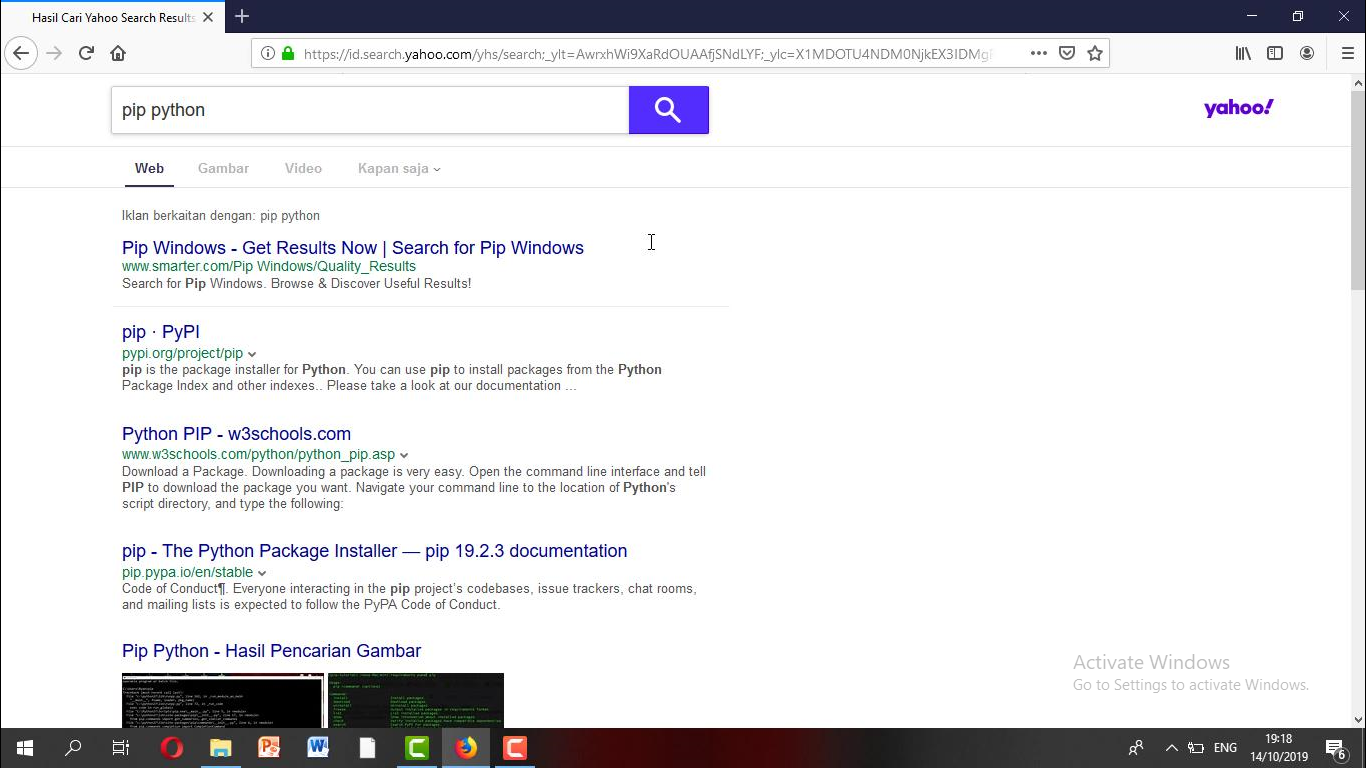
\includegraphics[scale=0.2]{gambar/pip1.png}
    \caption{Gambar1}
    \label{fig:my_label}
\end{figure}
\item Lalu klik installation,seperti yang ditunjuk tanda panah.
\begin{figure}[h]
    \centering
    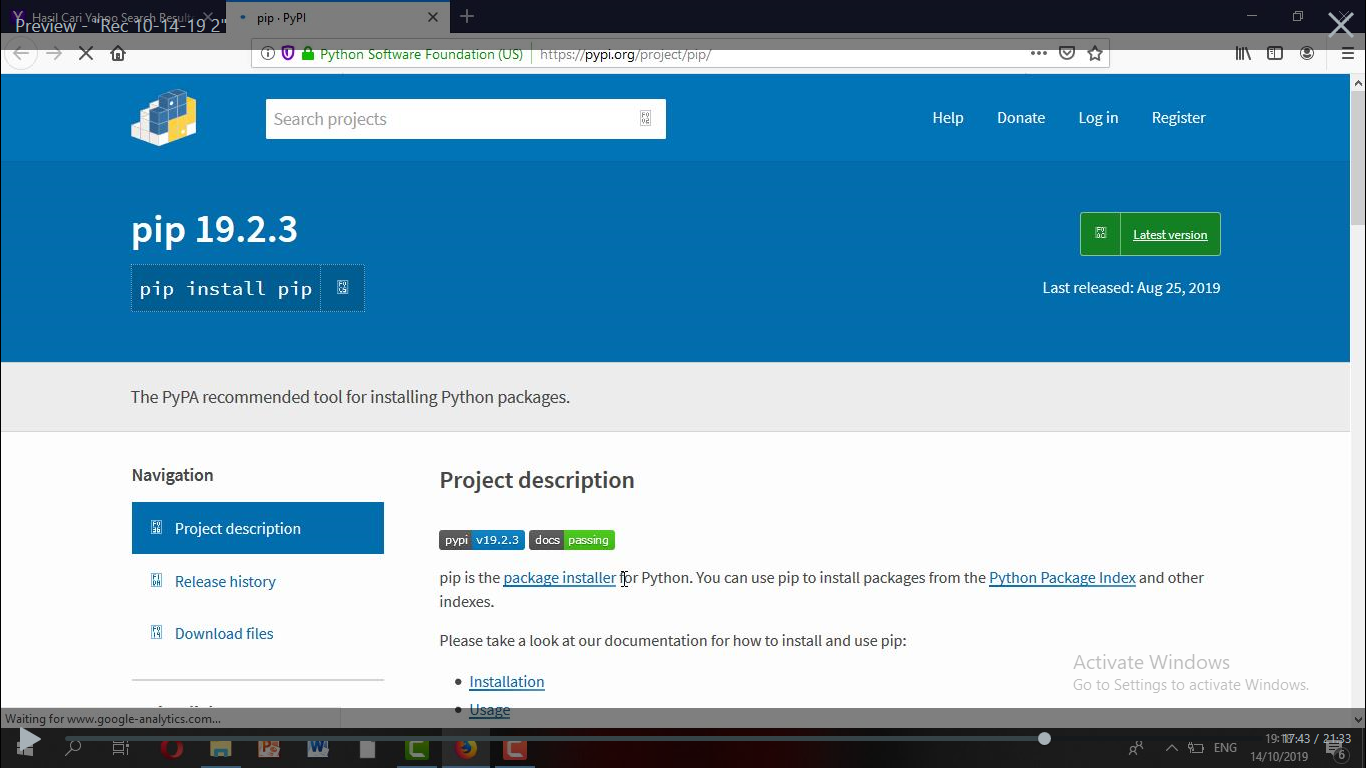
\includegraphics[scale=0.2]{gambar/pip2.png}
    \caption{Gambar2}
    \label{fig:my_label}
\end{figure}
\item Kemudian klik get.pip.py seperti yang ditunjuk tanda panah dibawah ini, lalu klik ok.
\begin{figure}[h]
    \centering
    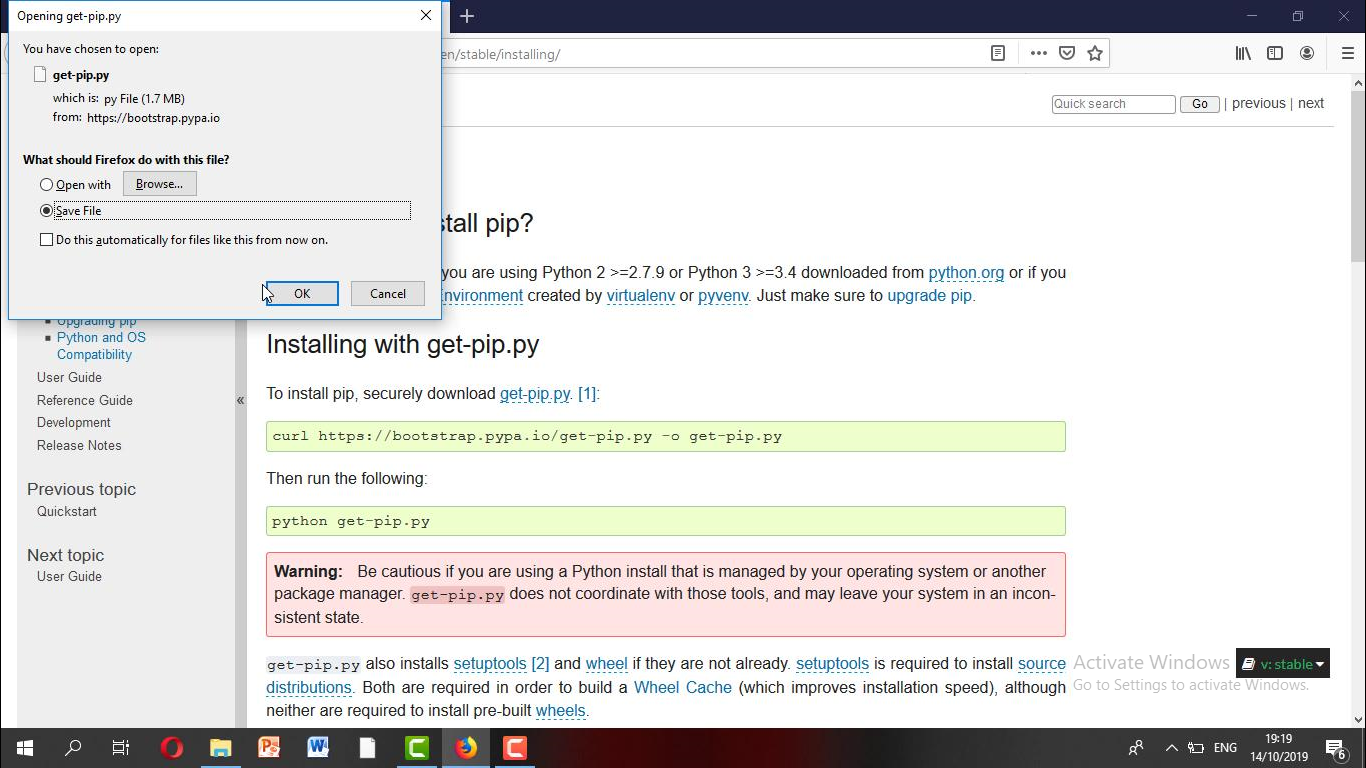
\includegraphics[scale=0.2]{gambar/pip3.png}
    \caption{Gambar3}
    \label{fig:my_label}
\end{figure}
\item Setelah itu buka cmd
\begin{figure}[h]
    \centering
    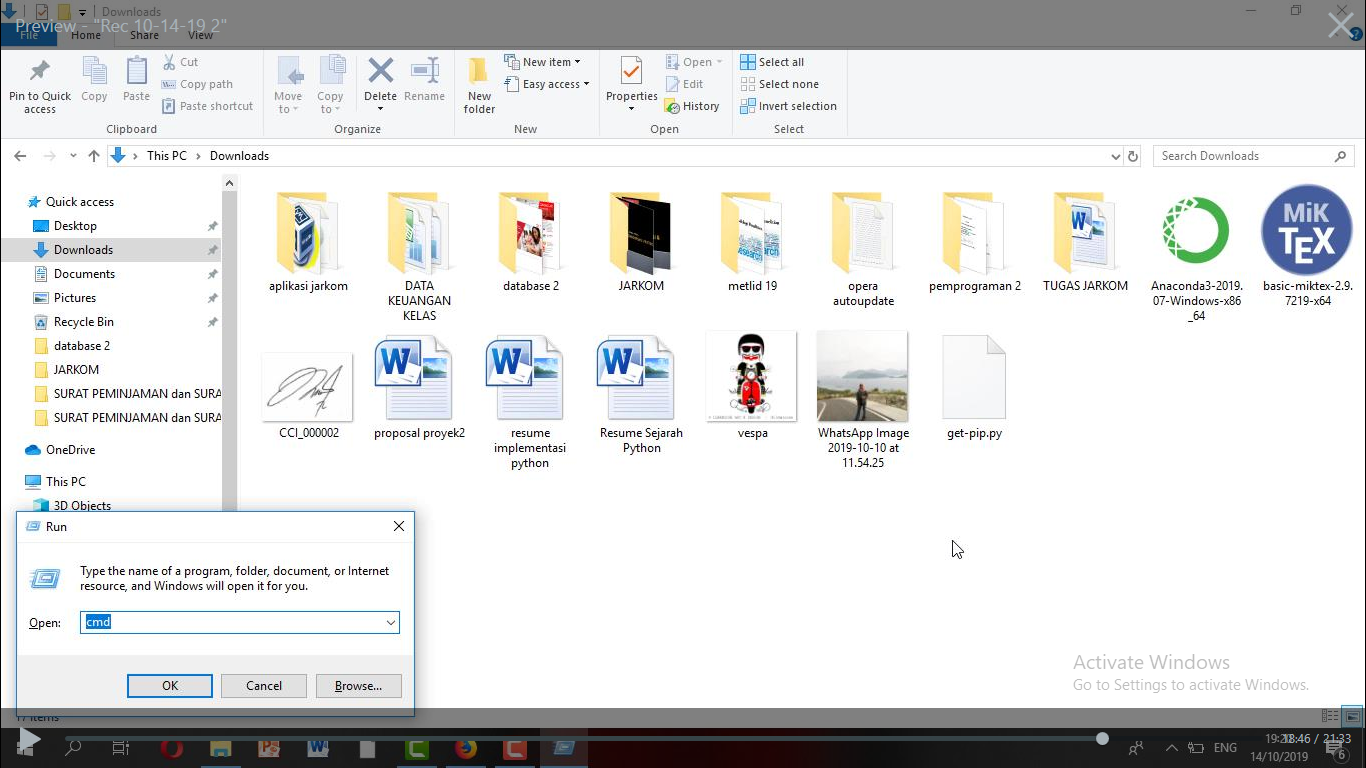
\includegraphics[scale=0.2]{gambar/pip4.png}
    \caption{Gambar4}
    \label{fig:my_label}
\end{figure}
\item Lalu ketik  python get.pip.py
\begin{figure}[h]
    \centering
    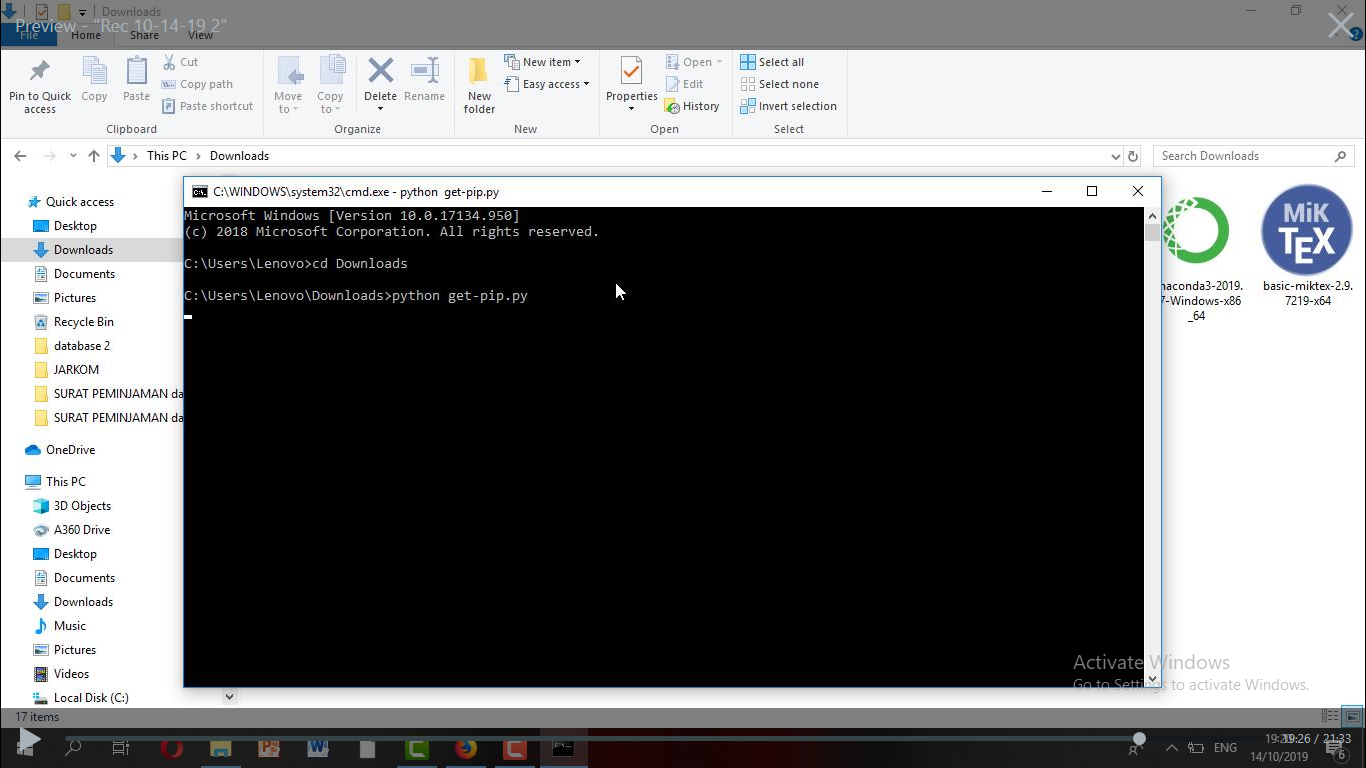
\includegraphics[scale=0.2]{gambar/pip5.png}
    \caption{Gambar5}
    \label{fig:my_label}
\end{figure}
\item Jika tampilanya sudah seperti gambar yang dibawah ini, maka sudah selesai
\begin{figure}[h]
    \centering
    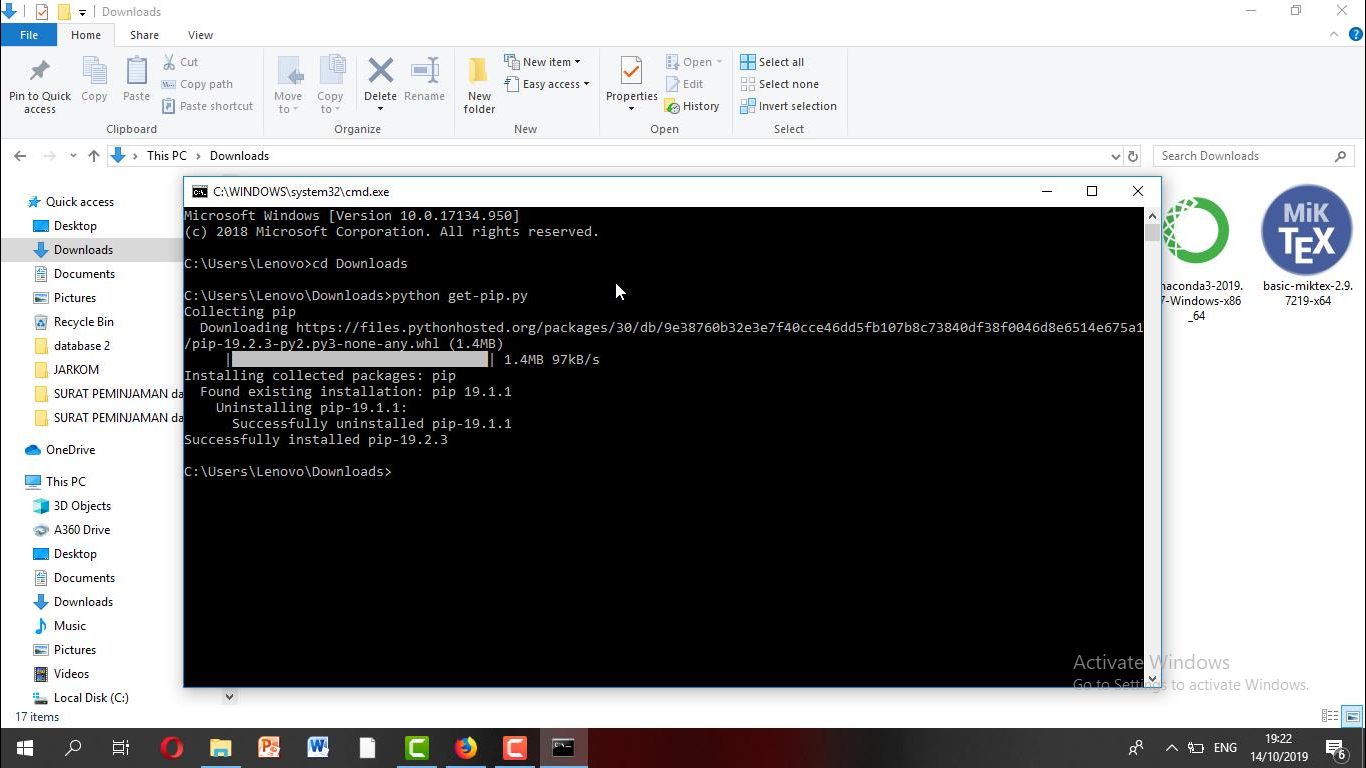
\includegraphics[scale=0.2]{gambar/pip6.png}
    \caption{Gambar6}
    \label{fig:my_label}
\end{figure}
\end{enumerate}